\documentclass[x11names, 10pt]{beamer}

\usefonttheme{professionalfonts}

\usepackage[T1]{fontenc}
\usepackage{newpxtext}
\usepackage{newpxmath}
\usepackage{algorithm}
\usepackage{algorithmic}
\usepackage{amsmath}
\usepackage{bm}
\usepackage{centernot}
\usepackage{natbib}
\usepackage[absolute, overlay]{textpos} % showboxes to show boxes.
\usepackage{tikz}
\usepackage{wasysym}
\usepackage{xfrac}

% Sets.
\newcommand*{\M}{\mathcal{M}}
\newcommand*{\Reals}{\mathbb{R}}
\renewcommand*{\S}{\mathcal{S}}
\newcommand*{\X}{\mathcal{X}}
\newcommand*{\Y}{\mathcal{Y}}
\newcommand*{\Yh}{\hat{\Y}}

% Operators.
\DeclareMathOperator{\bnabla}{\bm{\nabla}}
\DeclareMathOperator{\E}{\mathrm{E}}
\renewcommand*{\O}{\mathcal{O}}
\DeclareMathOperator{\Prob}{\mathrm{P}}
\DeclareMathOperator*{\argmax}{arg\,max}
\renewcommand*{\d}[2]{\dfrac{d #1}{d #2}}
\newcommand*{\p}[2]{\dfrac{\partial #1}{\partial #2}}
\DeclareMathOperator{\softmax}{\mathrm{softmax}}

% Matrices.
\newcommand*{\V}{\mathbf{V}}
\newcommand*{\W}{\mathbf{W}}

% Vectors.
\renewcommand*{\b}{\mathbf{b}}
\newcommand*{\cc}{\mathbf{c}}
\newcommand*{\e}{\mathbf{e}}
\newcommand*{\f}{\mathbf{f}}
\newcommand*{\h}{\mathbf{h}}
\newcommand*{\SIGMA}{\bm{\sigma}}
\newcommand*{\THETA}{\bm{\theta}}
\renewcommand*{\v}{\mathbf{v}}
\newcommand*{\w}{\mathbf{w}}
\newcommand*{\x}{\mathbf{x}}
\newcommand*{\dx}{\mathbf{dx}}
\newcommand*{\y}{\mathbf{y}}
\newcommand*{\dy}{\mathbf{dy}}
\newcommand*{\yh}{\hat{\y}}
\newcommand*{\z}{\mathbf{z}}

% LaTeX things.
\renewcommand{\thefootnote}{\fnsymbol{footnote}}

% Links.
\newcommand*{\bluelink}[2]{\href{#1}{\textcolor{blue}{#2}}}
\newcommand*{\blueurl}[1]{\textcolor{blue}{\url{#1}}}

% TikZ commands.

% Entry on a horizontal arrow.
\newcommand{\entry}[2]{
    \draw [thick] (#2, \pos - 0.2) -- (#2, \pos + 0.2) node [below, pos=0] {#1};
}

% Args: top left x coordinate, top left y coordinate, size
\newcommand{\featuremap}[3]{\grid{green}{#1}{#2}{#3}}
% Args: top left x coordinate, top left y coordinate
\newcommand{\filter}[2]{\grid{red}{#1}{#2}{5}}
% Args: color, top left x coordinate, top left y coordinate, size
\newcommand{\grid}[4]{
    \fill [#1!20] (#2, #3) rectangle (#2 + #4, #3 - #4);
    \draw [image] (#2, #3) grid (#2 + #4, #3 - #4);
    \draw [very thick] (#2, #3) rectangle (#2 + #4, #3 - #4);
}
% Args: top left x coordinate, top left y coordinate
\newcommand{\image}[2]{\grid{blue}{#1}{#2}{20}}
\newcommand{\mlpblock}{
    \begin{block}{}
        \vspace{-1em}
        \begin{align*}
            \hat{y}_k &= \sum_{j=1}^n v_{kj} \sigma\left(\sum_{i=1}^q w_{ji} x_i + b_j\right) + c_k,
            \quad
            k = 1, \ldots, p \\
            L(\y, \yh) &= \frac{1}{p} \sum_{k=1}^p (y_k - \hat{y}_k)^2, \qquad
            \p{L}{\hat{y}_k} = \frac{2 (\hat{y}_k - y_k)}{p}
        \end{align*}
    \end{block}
}
\newcommand{\scale}[2]{
    \draw [Latex-Latex, very thick] (-3.6, \pos) -- (3.6, \pos)
    node [left, pos=0, align=right] {#1}
    node [right, pos=1, align=left] {#2};
}

% Make a variant of \vdots without the top vertical space.
\makeatletter
\DeclareRobustCommand{\vvdots}{%
    \vbox{
        \baselineskip4\p@\lineskiplimit\z@
        \kern-\p@
        \hbox{.}\hbox{.}\hbox{.}
    }
}
\makeatother

% Theme settings.
\usetheme{Frankfurt}
\usefonttheme{serif}

% Other Beamer settings.
\setbeamercovered{transparent}
\AtBeginSection[]{%
    \begin{frame}{Outline}
        \tableofcontents[currentsection]
    \end{frame}
}

% TikZ commands.
\usetikzlibrary{arrows.meta, positioning}

\tikzset{
    onslide/.code args={<#1>#2}{
        \only<#1>{\pgfkeysalso{#2}} % \pgfkeysalso doesn't change the path
    }
}
\tikzset{
    temporal/.code args={<#1>#2#3#4}{
        % \pgfkeysalso doesn't change the path
        \temporal<#1>{\pgfkeysalso{#2}}{\pgfkeysalso{#3}}{\pgfkeysalso{#4}}
    }
}

\tikzstyle{activation} = [draw, block, fill=green!20]
\tikzstyle{affine} = [draw, block, fill=blue!20]
\tikzstyle{block} = [minimum width=7mm, minimum height=7mm, thick, rectangle, rounded corners, font=\small, inner sep=2.5pt]
\tikzstyle{image} = [step=1.5mm, gray, very thin]
\tikzstyle{io} = [neuron, fill=yellow!20]
\tikzstyle{io mini} = [neuron mini, fill=yellow]
\tikzstyle{io mini off} = [neuron mini, fill=yellow!20, draw=black!20]
\tikzstyle{neuron} = [draw, minimum width=5mm, minimum height=5mm, thick, rectangle, rounded corners, inner sep=0pt, fill=red!20]
\tikzstyle{neuron mini} = [draw, minimum width=2mm, minimum height=2mm, circle, inner sep=0pt, fill=red]
\tikzstyle{neuron mini off} = [neuron mini, fill=red!20, draw=black!20]
\tikzstyle{path} = [-Latex, thick]
\tikzstyle{scalar} = [draw, block, fill=yellow!20, text height=1.5ex, text depth=0.25ex]

% Figures.
\graphicspath{{figures/}}

% Title, author, date, classification, etc.
\title{Machine learning \& neural network introduction}
\author[Kevin K. Chen]{%
    \texorpdfstring{%
        Kevin K. Chen \\
        \normalsize \href{%
            mailto:kkchen@ccrwest.org%
        }{%
            \textcolor{blue}{\texttt{kkchen@ccrwest.org}}%
        }%
    }{%
        Kevin K. Chen%
    }%
}
\institute[IDA/CCRL]{Institute for Defense Analyses \\ Center for Communications Research - La Jolla}
\date{February 20, 2018}

% Bibliography commands.
\bibliographystyle{plainnat}
\setcitestyle{round}

\includeonly{sections/cnn}

\begin{document}

\begin{frame}
    \maketitle
\end{frame}

\begin{frame}{Outline}
    \tableofcontents[hideallsubsections]
\end{frame}

%%% Local Variables:
%%% mode: latex
%%% TeX-master: "../nn"
%%% End:

% Will not offer expert knowledge on NNs in fluid dynamics (see APS; follow research)

\section[ML overview]{Machine learning overview}

\subsection{}

\begin{frame}
    \frametitle{What is machine learning?}

    \begin{block}{My definition}
        The study of computational algorithms
        \begin{itemize}
            \item that \alert{predict} outputs from inputs;
            \item whose behavior is determined by \alert{model parameters};
            \item that \alert{learn} how to make predictions by fitting (``training'') the model parameters to data;
            \item that \alert{iteratively} improve their model parameters via continual training.
        \end{itemize}
    \end{block}

    \begin{columns}
        \begin{column}{2.5in}
            Simplest example: linear regression
            \begin{itemize}
                \item Sort of: not iterative
                \item Predicts $y$ from $x$ via $y = ax + b$
                \item Two parameters: $a$, $b$
                \item Fitted to data
            \end{itemize}
        \end{column}
        \begin{column}{1.75in}
            \includegraphics{linear_regression}
        \end{column}
    \end{columns}
\end{frame}

\begin{frame}
    \frametitle{A (much) more complicated example}
    \begin{columns}
        \begin{column}{0.37\textwidth}
            \begin{block}{Image classification}
                A canonical problem: given an image, predict the correct label
            \end{block}
        \end{column}
        \begin{column}{0.63\textwidth}
            \includegraphics[width=\textwidth]{cifar10}
        \end{column}
    \end{columns}

    \begin{itemize}
        \item Roughly: if a human can do it, a computer should be able to too
        \item More rigorously: $\exists$ a mapping from image pixels to labels
        \begin{itemize}
            \item Mapping too difficult for humans to understand
            \item Let an algorithm model it
        \end{itemize}
    \end{itemize}
\end{frame}

\begin{frame}
    \frametitle{An image classification solution}

    \begin{columns}
        \begin{column}{0.7\textwidth}
            ResNet-152: a 152-layer convolutional neural network with 11.3 billion multiply/adds! \citep{He15}
            \begin{itemize}
                \item Trained on ImageNet data: 14,197,122 images
                \item Iterative training
                \begin{itemize}
                    \item 600,000 training iterations
                    \item At each iteration, model parameters updated based on \emph{mini-batch} of 256 images
                \end{itemize}
                \item Won multiple image classification competitions
            \end{itemize}
        \end{column}
        \begin{column}{0.3\textwidth}
            \includegraphics[width=\textwidth]{resnet}
        \end{column}
    \end{columns}
\end{frame}
% Universal approximation
% Quick thing on decision trees

%%% Local Variables:
%%% mode: latex
%%% TeX-master: "../nn"
%%% End:

\section{Loss}

\subsection{}

\begin{frame}
    \frametitle{How accurate is a model?}
    
\end{frame}

%%% Local Variables:
%%% mode: latex
%%% TeX-master: "../nn"
%%% End:

\section{Dense neural networks}

\subsection{}

\begin{frame}
    \frametitle{The neuron: equations}

    Consider an input $\x \in \Reals^q$.
    \begin{block}{}
        Consider some \emph{weight vector} $\w \in \Reals^q$ and \emph{bias} $b \in \Reals$.
        The mapping
        \begin{align*}
            g &: \Reals^q \to \Reals \\
            &\hspace{1.25ex} \x \mapsto \w \cdot \x + b
        \end{align*}
        is an \alert{affine transformation}.
    \end{block}
    \pause

    Consider a generally nonlinear \alert{activation function} $\sigma: \Reals \to \Reals$.

    \begin{block}{}
        An (artifical) \alert{neuron} is the function $\phi = \sigma \circ g$, i.e.,
        \begin{align*}
            \phi &: \Reals^q \to \Reals \\
            &\hspace{1.25ex} \x \mapsto \sigma(\w \cdot \x + b)
        \end{align*}
    \end{block}
    \pause

    \begin{itemize}
        \item Historically, artificial neuron modeled on biological neurons
        \begin{itemize}
            \item Bio neuron triggers impulse by nonlinear function of inputs
        \end{itemize}
        \item Today, relation is largely only conceptual/philosophical
    \end{itemize}
\end{frame}

\begin{frame}
    \frametitle{The neuron: geometric interpretation}

    \begin{itemize}
        \item Activation functions $\sigma(x)$ typically most ``interesting'' at $x = 0$
        \item For neuron $\phi(x) = \sigma(\w \cdot \x + b)$, \textcolor{Green4}{hyperplane} $\w \cdot \x + b = 0$ is a natural boundary in $\X$
        \item Simple example:
        \begin{itemize}
            \item $\x =$ (sex, age, weight, height, LDL, HDL, exercise hrs/wk, smoker)
            \item $y =$ heart disease risk
            \item Medical intuition: larger risk for men, older, heavier, shorter, higher LDL, lower HDL, less exercise, smoker
            \item Geometric interpretation: draw \textcolor{Green4}{hyperplane} through $\Reals^8$ best separating \alert{high-risk} from \textcolor{blue}{low-risk}
        \end{itemize}
    \end{itemize}

    \centering
    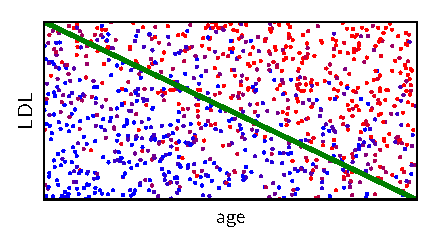
\includegraphics{plane}
\end{frame}

\begin{frame}
    \frametitle{Single hidden-layer neural network: vector equations}

    Consider $n$ neurons each taking in $\x \in \Reals^q$: given
    \begin{itemize}
        \item weight vectors $\w_k \in \Reals^q$, $k = 1, \ldots, n$,
        \item biases $b_k \in \Reals$, $k = 1, \ldots, n$,
    \end{itemize}
    \begin{block}{Hidden layer}
        \vspace{-1em}
        \begin{align*}
            z_k &= \sigma(\w_k \cdot \x + b_k), \quad k = 1, \ldots, n \\
            \z &= \begin{bmatrix} z_1 & \cdots & z_n \end{bmatrix} \in \Reals^n
        \end{align*}
    \end{block}
    \pause

    Let the model output $\y \in \Reals^p$ be affine transformations of $\z$: given
    \begin{itemize}
        \item weight vectors $\v_k \in \Reals^n$, $k = 1, \ldots, p$
        \item biases $c_k \in \Reals$, $k = 1, \ldots, p$
    \end{itemize}
    \begin{block}{Single hidden-layer dense neural network}
        \vspace{-1em}
        \begin{align*}
            y_k &= \v_k \cdot \z + c_k, \quad k = 1, \ldots, p \\
            \y &= \begin{bmatrix} y_1 & \cdots & y_p \end{bmatrix}
        \end{align*}
    \end{block}
\end{frame}

\begin{frame}
    \frametitle{Single hidden-layer neural network: figure}

    {
        \centering
        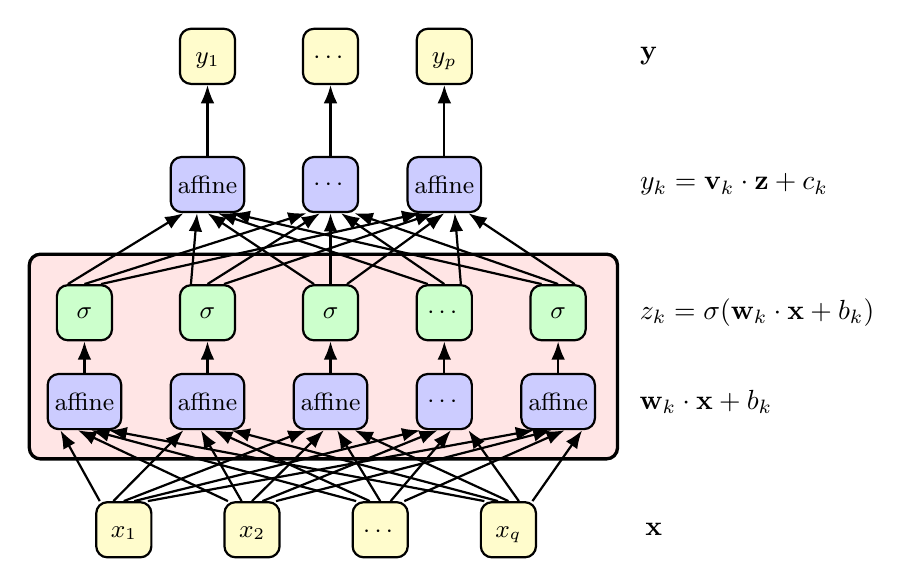
\begin{tikzpicture}[>=latex, node distance=9mm]
    % Inputs.
    \uncover<+->{
        \node (x1) [scalar] {$x_1$};
        \node (x2) [scalar, right=of x1] {$x_2$};
        \node (x3) [scalar, right=of x2] {$\cdots$};
        \node (x4) [scalar, right=of x3] {$x_q$};

        \node [right=1.25cm of x4] {$\x$};

    }

    \uncover<+->{
        % Hidden layer.
        \draw [very thick, rounded corners, fill=red!10]
        (-1.2, 0.9) rectangle (6.27, 3.5);

        % Hidden layer combinations.
        \node (affine x1) [affine, above=of x1, xshift=-5mm] {affine};
        \node (affine x2) [affine, right=6mm of affine x1] {affine};
        \node (affine x3) [affine, right=6mm of affine x2] {affine};
        \node (affine x4) [affine, right=6mm of affine x3] {$\cdots$};
        \node (affine x5) [affine, right=6mm of affine x4] {affine};

        \node [right=4.3mm of affine x5] {$\w_k \cdot \x + b_k$};
    }

    \uncover<+->{
        % Hidden layer activations.
        \foreach \i in {1, 2, 3, 5} {
            \node (sigma\i) [activation, above=4mm of affine x\i] {$\sigma$};
        }

        \node (sigma4) [activation, above=4mm of affine x4] {$\cdots$};

        \node [right=5.5mm of sigma5] {$z_k = \sigma(\w_k \cdot \x + b_k)$};
    }

    % Output combinations.
    \uncover<+->{
        \node (affine y1) [affine, above=of sigma2] {affine};
        \node (affine y2) [affine, above=of sigma3] {$\cdots$};
        \node (affine y3) [affine, above=of sigma4] {affine};

        \node [right=1.88cm of affine y3] {$y_k = \v_k \cdot \z + c_k$};
    }

    % Outputs.
    \uncover<+->{
        \node (y1) [scalar, above=of affine y1] {$y_1$};
        \node (y2) [scalar, above=of affine y2] {$\cdots$};
        \node (y3) [scalar, above=of affine y3] {$y_p$};

        \node [right=2cm of y3] {$\y$};
    }

    % Connections.

    \foreach \i/\a in {1/130, 2/110, 3/90, 4/70, 5/50} {
        % Inputs to affines.
        \foreach \j/\b in {1/230, 2/257, 3/283, 4/310} {
            \uncover<2->{\draw [path] (x\j.\a) -- (affine x\i.\b);}
        }

        % Hidden layer affines to activations.
        \uncover<3->{\draw [path] (affine x\i) -- (sigma\i);}
    }

    \foreach \j/\b in {1/120, 2/90, 3/60} {
        % Hidden layer activations to output affines.
        \foreach \i/\a in {1/230, 2/250, 3/270, 4/290, 5/310} {
            \uncover<4->{\draw [path] (sigma\i.\b) -- (affine y\j.\a);}
        }

        % Output affines to outputs.
        \uncover<5->{\draw [path] (affine y\j) -- (y\j);}
    }
\end{tikzpicture}

%%% Local Variables:
%%% mode: latex
%%% TeX-master: "../nn"
%%% End:

    }
    \vspace{0.5ex}

    Dense neural network, a.k.a.~feedforward neural network, a.k.a.~multi-layer perceptron
\end{frame}

\begin{frame}
    \frametitle{Single hidden-layer neural network: matrix equations}

    The equations are more compact in matrix form:
    \begin{itemize}
        \item Weight matrix $\W \in \Reals^{n \times q}$
        \item Bias vector $\b \in \Reals^n$
        \item Element-wise activation function
        \begin{align*}
            \SIGMA &: \Reals^n \to \Reals^n \\
            &\hspace{1.25ex} \begin{bmatrix} \xi_1 & \cdots & \xi_n \end{bmatrix} \mapsto
            \begin{bmatrix} \sigma(\xi_1) & \cdots & \sigma(\xi_n) \end{bmatrix}
        \end{align*}
    \end{itemize}

    \begin{block}{Hidden layer}
        \begin{equation*}
            \z = \SIGMA(\W \x + \b)
        \end{equation*}
    \end{block}
    \pause

    \begin{itemize}
        \item Weight matrix $\V \in \Reals^{q \times n}$
        \item Bias vector $\cc \in \Reals^q$
    \end{itemize}

    \begin{block}{Single hidden-layer dense neural network}
        \begin{equation*}
            \y = \V \z + \cc
        \end{equation*}
    \end{block}
\end{frame}

\begin{frame}
    \frametitle{Activation functions}
    \begin{block}{Why do neurons have nonlinear activation functions?}
        If $\sigma$ is linear (including the identity $\sigma(x) = x$, i.e. no activation), the neural network $\f : \x \mapsto \y$ is necessarily linear \\[1ex]
        For $\f$ to be nonlinear, \alert{activation functions must be nonlinear}!
    \end{block}

    In some sense, it doesn't even matter what $\sigma$ is, as long as it's nonlinear. \\[1ex]

    To be more particular, $\sigma$ should
    \begin{itemize}
        \item be fast to compute (will be called gazillions of times)
        \item not lead to vanishing or exploding gradients
    \end{itemize}
\end{frame}

\begin{frame}
    \frametitle{Common activation functions}
    \begin{columns}
        \begin{column}{2.5in}
            \begin{itemize}
                \item \textcolor{Green4}{Standard logistic/sigmoid function: $\sigma(x) = \dfrac{1}{1 + e^{-x}} = \dfrac{\tanh(x) + 1}{2}$}
                \begin{itemize}
                    \item Used to be preferred
                    \item Now thought to be too slow
                    \item Suffers from vanishing gradients
                \end{itemize}
                \item \textcolor{blue}{Rectified linear unit (ReLU): $\sigma(x) = \max(0, x)$}
                \begin{itemize}
                    \item Most common, but suffers from vanishing gradients
                \end{itemize}
            \end{itemize}
        \end{column}
        \begin{column}{2in}
            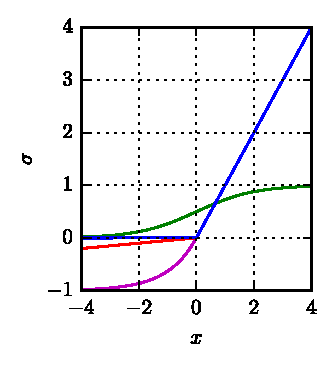
\includegraphics{activations}
        \end{column}
    \end{columns}

    % Ugly hack to make the bullets line up.
    \begin{columns}
        \begin{column}{4.7in}
            \begin{itemize}
                \item \textcolor{red}{Leaky/parametric ReLU} \citep{MaasICML13,He15a}:
                \textcolor{red}{
                    $\sigma(x) = \begin{cases}
                        x &\mid x \ge 0 \\
                        \alpha x &| x < 0
                    \end{cases}$
                }
                \item \textcolor{Magenta3}{Exponential linear unit (ELU)} \citep{ClevertICLR16}:
                \textcolor{Magenta3}{
                    $\sigma(x) = \begin{cases}
                        x &\mid x > 0 \\
                        \alpha (e^x - 1) &\mid x \le 0
                    \end{cases}$
                }
            \end{itemize}
        \end{column}
    \end{columns}
\end{frame}

\begin{frame}
    \frametitle{Deep neural networks}

    No reason to stop at only one hidden layer!

    \vspace{1mm}
    \begin{tikzpicture}[node distance=6mm]
    % Layer 1.
    \uncover<2->{\node (n11) [neuron] {};}

    \foreach \i in {1, ..., 4} {
        \pgfmathtruncatemacro{\j}{\i + 1}
        \uncover<2->{\node (n1\j) [neuron, right=of n1\i] {};}

        % Inputs.
        \node (x\i) [io, below=of n1\i, xshift=6mm] {};
        % Layer 2.
        \uncover<3->{\node (n2\i) [neuron, above=of n1\i, xshift=6mm] {};}
    }

    \foreach \i in {1, ..., 3} {
        % Invisible layer 3.
        \node (n3\i) [minimum width=5mm, above=of n2\i, xshift=5mm] {};
        % Invisible layer 4.
        \node (n4\i) [above=4mm of n3\i] {};
    }

    % Etc.
    \uncover<4->{\node (etc) [above=8mm of n22, xshift=6mm] {$\vdots$};}

    \uncover<5->{
        \node (nl1) [neuron, above=of etc, xshift=-6mm] {};
        \node (nl2) [neuron, right=of nl1] {};
    }

    % Outputs.
    \uncover<6->{
        \node (y2) [io, above=of nl1] {};
        \node (y3) [io, above=of nl2] {};
        \node (y1) [io, left=of y2] {};
        \node (y4) [io, right=of y3] {};
    }

    \node [right=of x4, xshift=5.5mm] {$\x \in \Reals^q$};
    \uncover<2->{
        \node [right=of n15] {$\z_1 = \SIGMA(\W_1 \x + \b_1) \in \Reals^{n_1}$};
    }
    \uncover<3->{
        \node [right=of n24, xshift=5.4mm] {$\z_2 = \SIGMA(\W_2 \z_1 + \b_2) \in \Reals^{n_2}$};
    }
    \uncover<4->{
        \node [right=of n33, yshift=-2mm, xshift=1.64cm] {$\vdots$};
        \node [right=of etc, yshift=-1mm, xshift=2.28cm] {$\z_i = \SIGMA(\W_i \z_{i-1} + \b_i) \in \Reals^{n_i}$};
    }
    \uncover<5->{
        \node [right=of n43, yshift=5mm, xshift=1.76cm] {$\vdots$};
        \node [right=of nl2, xshift=1.68cm] {$\z_l = \SIGMA(\W_l \z_{l-1} + \b_l) \in \Reals^{n_l}$};
    }
    \uncover<6->{\node [right=of y4, xshift=5.4mm] {$\y = \V \z_l + \c \in \Reals^p$};}

    \foreach \i in {1, ..., 4} {
        \foreach \j in {1, ..., 5} {
            \uncover<2->{\draw [path] (x\i.90) -- (n1\j.270);}
            \uncover<3->{\draw [path] (n1\j.90) -- (n2\i.270);}
        }

        \foreach \j in {1, ..., 3} {
            \uncover<4->{\draw [path] (n2\i.90) -- (n3\j.270);}
        }
    }

    \foreach \i in {1, 2} {
        \foreach \j in {1, ..., 3} {
            \uncover<5->{\draw [path] (n4\j.90) -- (nl\i.270);}
        }

        \foreach \j in {1, ..., 4} {
            \uncover<6->{\draw [path] (nl\i.90) -- (y\j.270);}
        }
    }
\end{tikzpicture}

%%% Local Variables:
%%% mode: latex
%%% TeX-master: "../nn"
%%% End:

    \vspace{1mm}

    Common but not necessary for $\SIGMA$ to be the same in each layer
\end{frame}

\begin{frame}
    \frametitle{Why is deep better than wide?}
    \begin{itemize}
        \item Depth: \# layers
        \item Width: \# neurons in each layer (need not be fixed)
    \end{itemize}
    \pause

    Neural network with $\sigma = \text{ReLU}$ is piecewise linear function
    \begin{itemize}
        \item \alert{Expressivity} of ReLU network measured by \# linear pieces
        \item For fixed width $w$ and depth $l$, \alert{$\max \text{expressivity} \sim w^l$} \citep{Pascanu13,MontufarNIPS14,Chen16}
        \item In comparison, $\alert{\text{\# parameters}} = (q + 1) n_1 + (n_1 + 1) n_2 + \cdots + (n_{l-1} + 1) n_l + (n_l + 1) p \approx \alert{w^2 l}$
    \end{itemize}
    \pause

    Common for layers closer to the input to be wider
    \begin{itemize}
        \item Closer to the input $\implies$ more expressive power over output \citep{RaghuICML17}
    \end{itemize}
    \pause

    \begin{block}{}
        Depth is (arguably) the key reason for the ML/AI explosion in the last decade.
        Recall ResNet---152 layers deep!
    \end{block}
\end{frame}

\begin{frame}
    \frametitle{%
        Example: $\Reals^2 \to \Reals$ ripple\footnote{%
            Code: \blueurl{https://goo.gl/Yv8CW3}.
            Trained to convergence: $\sim8 \cdot 10^7$ samples.%
        }%
    }
    \begin{columns}
        \begin{column}{0.5\textwidth}
            \centering
            \includegraphics[width=1.85in]{ripple} \\
            Ground truth: $y = \dfrac{\cos(r)}{e^{0.4 (r - 8)} + 1}$
        \end{column}
        \hfill
        \pause
        \begin{column}{0.5\textwidth}
            \centering
            \includegraphics[width=1.85in]{ripple_1layer} \\
            1 layer, 50 neurons, \\ 201 parameters: $R = 8.1 \cdot 10^{-2}$
        \end{column}
    \end{columns}
    \pause

    \begin{columns}
        \begin{column}{0.5\textwidth}
            \centering
            \includegraphics[width=1.85in]{ripple_2layer} \\
            2 layers, 17--8 neurons, \\ 204 parameters: $R = 4.9 \cdot 10^{-3}$
        \end{column}
        \hfill
        \pause
        \begin{column}{0.5\textwidth}
            \centering
            \includegraphics[width=1.85in]{ripple_3layer} \\
            3 layers, 15--7--4 neurons, \\ 194 parameters: $R = 1.6 \cdot 10^{-3}$
        \end{column}
    \end{columns}
\end{frame}

\begin{frame}
    \frametitle{What can dense neural networks model?}
    \begin{block}{Universal approximation theorem}
        Anything, basically, if $\text{width} \to \infty$
        \begin{itemize}
            \item Depth not required; 1 hidden layer is enough
        \end{itemize}
    \end{block}

    Some mild conditions required.
    Limitations on $\sigma$:
    \begin{itemize}
        \item $\sigma$ is sigmoid \citep{CybenkoMCSS89,HornikNN89,HornikNN91}
        \item $\sigma$ can be ReLU, polynomial, Gaussian, etc. \citep{SonodaACHA}
    \end{itemize}
\end{frame}

%%% Local Variables:
%%% mode: latex
%%% TeX-master: "../nn"
%%% End:

\section{Training}

\subsection{}

\begin{frame}
    \frametitle{Recap \& training objective}

    What we have so far
    \begin{itemize}
        \item<+-> A neural network $\f$
        \begin{itemize}
            \item User-selected \alert{architecture} (\# layers, \# neurons/layer, activations)
            \item Behavior set by thousands--billions of \alert{parameters} (weights \& biases) $\THETA = (\W_1, \b_1, \W_2, \b_2, \ldots)$
            \item \alert{Predicts} $\yh$ from $\x$ via $\yh = \f(\x; \THETA)$
            \item \alert{Universal approximation theorem}: $\f$ can model anything if $\THETA$ big enough
        \end{itemize}
        \item<+-> Gobs of \alert{data} pairs $\S = \{(\x, \y)\}$
        \item<+-> User-selected \alert{loss function} $L(\y, \yh)$
        \item<+-> Desire to minimize \alert{model risk} $R(\f; \THETA; \S) = \E_{(\x, \y) \in \S}(L(\y, \f(\x; \THETA)))$
    \end{itemize}

    \begin{block}{Training objective}<+->
        Iterate on $\THETA$ to minimize $R(\f; \THETA; \S)$
    \end{block}

    \begin{block}{Methodology}<+->
        Compute $\p{R}{\THETA}$ and use gradient descent
    \end{block}
\end{frame}

\begin{frame}
    \frametitle{Backpropagation}

    \uncover<+->{
        Since model risk $R$ is average over data of losses $L(\y, \f(\x; \THETA))$, gradient $\p{R}{\THETA}$ is average over data of $\p{L}{\THETA}$
    }

    \begin{block}{}<+->
        Backpropagation is how to compute $\p{L}{\THETA}$.
        It's literally just the chain rule.
    \end{block}

    \begin{itemize}
        \item<+-> Technique: symbolically pre-compute every element of $\p{L}{\THETA}$ via chain rule (one-time work)
        \begin{itemize}
            \item Software does this automatically
            \item Tedious, so we'll see one brief example next
        \end{itemize}
        \item<+-> When new datum $(\x, \y)$ arrives, plug in to get $\p{L}{\THETA}$
        \begin{itemize}
            \item Just multiplies, adds, \& activation functions---lightning fast
        \end{itemize}
        \item<+-> Average over data to get $\p{R}{\THETA}$
    \end{itemize}
\end{frame}

\begin{frame}
    \frametitle{Backpropagation example (1/3)}
    \begin{itemize}
        \item Single hidden-layer dense $\Reals^q \to \Reals^p$ neural network
        \item $n$ neurons with ReLU activation in hidden layer
        \item Mean squared error loss
    \end{itemize}
    \pause

    \begin{block}{}
        \vspace{-1em}
        \begin{align*}
            \hat{y}_k &= \sum_{j=1}^n v_{kj} \sigma\left(\sum_{i=1}^q w_{ji} x_i + b_j\right) + c_k,
            \quad
            k = 1, \ldots, p \\
            L(\y, \yh) &= \frac{1}{p} \sum_{k=1}^p (y_k - \hat{y}_k)^2
        \end{align*}
    \end{block}
    \pause

    Note: for ReLU $\sigma$, $\d{\sigma}{x} = H(x)$, the Heaviside step function

    \begin{equation*}
        \p{L}{\hat{y}_k} = \frac{2 (\hat{y}_k - y_k)}{p}
    \end{equation*}
\end{frame}

\begin{frame}
    \frametitle{Backpropagation example (2/3)}

    \begin{block}{}
        \vspace{-1em}
        \begin{align*}
            \hat{y}_k &= \sum_{j=1}^n v_{kj} \sigma\left(\sum_{i=1}^q w_{ji} x_i + b_j\right) + c_k,
            \quad
            k = 1, \ldots, p \\
            L(\y, \yh) &= \frac{1}{p} \sum_{k=1}^p (y_k - \hat{y}_k)^2, \qquad
            \p{L}{\hat{y}_k} = \frac{2 (\hat{y}_k - y_k)}{p}
        \end{align*}
    \end{block}
    \pause

    \begin{align*}
        \p{L}{v_{kj}} &= \p{L}{\hat{y}_k} \p{\hat{y}_k}{v_{kj}}
        = \frac{2 (\hat{y}_k - y_k)}{p} \sigma\left(\sum_{i=1}^q w_{ji} x_i + b_j\right) \\
        \pause
        \p{L}{c_k} &= \p{L}{\hat{y}_k} \p{\hat{y}_k}{c_k}
        = \frac{2 (\hat{y}_k - y_k)}{p}
    \end{align*}
\end{frame}

\begin{frame}
    \frametitle{Backpropagation example (3/3)}

    \begin{block}{}
        \vspace{-1em}
        \begin{align*}
            \hat{y}_k &= \sum_{j=1}^n v_{kj} \sigma\left(\sum_{i=1}^q w_{ji} x_i + b_j\right) + c_k,
            \quad
            k = 1, \ldots, p \\
            L(\y, \yh) &= \frac{1}{p} \sum_{k=1}^p (y_k - \hat{y}_k)^2, \qquad
            \p{L}{\hat{y}_k} = \frac{2 (\hat{y}_k - y_k)}{p}
        \end{align*}
    \end{block}
    \pause

    \begin{align*}
        \p{L}{w_{ji}} &= \sum_{k=1}^p \p{L}{\hat{y}_k} \p{\hat{y}_k}{w_{ji}}
        = \sum_{k=1}^p \frac{2 (\hat{y}_k - y_k)}{p} v_{kj} H\left(\sum_{i=1}^q w_{jl} x_l + b_j\right) x_i \\
        \pause
        \p{L}{b_j} &= \sum_{k=1}^p \p{L}{\hat{y}_k} \p{\hat{y}_k}{b_j}
        = \sum_{k=1}^p \frac{2 (\hat{y}_k - y_k)}{p} v_{kj} H\left(\sum_{i=1}^q w_{jl} x_l + b_j\right)
    \end{align*}

    \ldots You get the point.
\end{frame}

\begin{frame}[t]
    \frametitle{The trouble with gradient-based optimization}

    Gradient-based methods \citep{PressNR} seek local minima \\[1ex]

    The usual case:
    \begin{itemize}
        \item $\exists$ global minimization methods, but very slow
        \item Direct gradient descent usually bad
        \item Better methods: conjugate gradient, quasi-Newton
        \item \alert{Easily falls into non-global minima}
    \end{itemize}

    \begin{textblock}{6}(9, 11)
        \includegraphics[width=\textwidth]{minima}
    \end{textblock}

    \pause

    For neural networks:
    \begin{itemize}
        \item Given data set $\S = \{(\x_i, \y_i)\}$ with enormous $|\S|$
        \item Want to find $\THETA$ to minimize approximate model risk $\displaystyle R(\f; \THETA; \S) = \frac{1}{|\S|} \sum_{(\x, \y) \in \S} L(\y, \f(\x; \THETA))$
        \item \alert{Intractable}
    \end{itemize}
\end{frame}

\begin{frame}
    \frametitle{Stochastic gradient descent \& mini-batching}
    \begin{algorithmic}[1]
        \uncover<+->{\FOR{$\text{epoch} = 1, \ldots, n_\text{epochs}$}}
        \uncover<+->{\STATE Randomize the data order of $\S$}
        \uncover<+->{\WHILE{not done with $\S$}}
        \uncover<+->{\STATE Peel off the next $k \ll |\S|$ elements of $\S$ into the \alert{mini-batch} $\M$}
        \uncover<+->{
            \STATE \label{item:gradient}
            Compute $\h = \p{R(\f; \THETA; \M)}{\THETA}$ using only the mini-batch $\M$
        }
        \uncover<+->{
            \STATE Take a small step against the gradient: $\THETA \leftarrow \THETA - \alpha\h$ with $0 < \alpha \ll 1$
        }
        \uncover<3->{\ENDWHILE}
        \ENDFOR
    \end{algorithmic}
    \vspace{1ex}

    \uncover<+->{Terminology:}
    \begin{itemize}[<.->]
        \item \alert{Learning rate}: $\alpha$
        \item \alert{Mini-batch size}: $k = |\M|$ (often just called \emph{batch size})
        \item \alert{Iteration}: a single gradient update
        \item \alert{Epoch}: a complete pass through the data
    \end{itemize}
\end{frame}

\begin{frame}
    \frametitle{Why stochastic gradient descent \& mini-batching?}
    It kills two birds with one stone

    \begin{block}{Tractability}
        \textcolor{red}{Gradient descent}: intractable to compute gradient $\p{R(\f; \THETA; \S)}{\THETA}$ when $|\S| \approx \dim(\THETA) = \O(10^3 \text{--} 10^{10})$ \\[1ex]
        \textcolor{blue}{SGD}: $\p{R(\f; \THETA; \M)}{\THETA}$ tractable when $|\M| = \O(10^1 \text{--} 10^3)$
    \end{block}

    \begin{block}{Global minimization}
        \textcolor{red}{Gradient descent}: easily falls into local minima \\[1ex]
        \textcolor{blue}{SGD}: stochastic because it takes gradient steps based on random small mini-batches
        \begin{itemize}
            \item Over long-run average, SGD mimics true gradient using all data
            \item In short-run, stochasticity gives SGD a chance to climb out of local minima if needed
        \end{itemize}
    \end{block}
\end{frame}

\begin{frame}
    \frametitle{SGD-based optimizers}
    \uncover<+->{Issues with vanilla SGD}
    \begin{itemize}
        \item In $\Reals^n$ with $n \gg 1$, most critical points are saddle points
        \item SGD easily gets stuck in saddle points
        \item In gradient step $\THETA \leftarrow \THETA - \alpha \bnabla R$, need to decay learning rate $\alpha$
    \end{itemize}

    \uncover<+->{Better alternatives}
    \begin{itemize}[<+->]
        \item<.-> Momentum: $\THETA \leftarrow \THETA - \alpha \bnabla R + \eta \mathbf{\Delta}\THETA$---encourages continuing previous update \citep{RumelhartNature86}
        \item RMSprop: divide learning rate by mean of recent gradient norms \citep{TielemanRMSProp}
        \item Adagrad: each parameter has own learning rate determined by its gradients \citep{DuchJMLR11}
        \item Adadelta: improves Adagrad by making learning rate decay less aggressive \citep{Zeiler12}
        \item \alert<+->{Adam}: adaptive learning rate \& momentum \citep{KingmaICLR15}
    \end{itemize}

    \uncover<.->{Short: use Adam; it's generally best and works great out-of-the-box}
\end{frame}

\begin{frame}
    \frametitle{Mini-batch size}

    Mini-batch size not a random decision; can have huge effects on training
    \begin{itemize}
        \item Mini-batch size usually integer power of 2---better GPU optimization
        \item $\text{Stochasticity} \sim \dfrac{\text{learning rate}}{(\text{mini-batch size}) (1 - \text{momentum})}$ \citep{SmithNIPS17}
        \item Historically, $\text{size} = 16 \text{--} 256$ common
        \item Growing trend toward extremely large (e.g., 8,192+) sizes
    \end{itemize}
    \pause

    Choosing mini-batch size
    \begin{itemize}
        \item Smaller: more stochastic
        \begin{itemize}
            \item Better at escaping non-global minima
        \end{itemize}
        \item Larger: less stochastic
        \begin{itemize}
            \item Better at converging to deep, narrow minima
            \item Faster---better GPU optimization
            \item But limited by available GPU memory
        \end{itemize}
    \end{itemize}
\end{frame}

\begin{frame}
    \frametitle{Initializing the weights and biases}

    \begin{itemize}
        \item Common approach: initialize weights by Glorot uniform \citep{GlorotAISTATS10}
        \begin{itemize}
            \item Basically, intelligently scaled uniform distribution
        \end{itemize}
        \item Initialize biases to 0
        \item Random initialization helps optimizer find initial directions
        \item Note: every training invocation gives different result!
        \begin{itemize}
            \item Manually set pseudorandom seed if reproducibility required
        \end{itemize}
    \end{itemize}
\end{frame}

\begin{frame}
    \frametitle{Underfitting and overfitting}

    \begin{alertblock}{Danger!}
        Neural networks are hard to fit, and real-life data are noisy.
        \emph{Underfitting} and \emph{overfitting} are your two biggest obstacles.
    \end{alertblock}
    \vspace{1ex}

    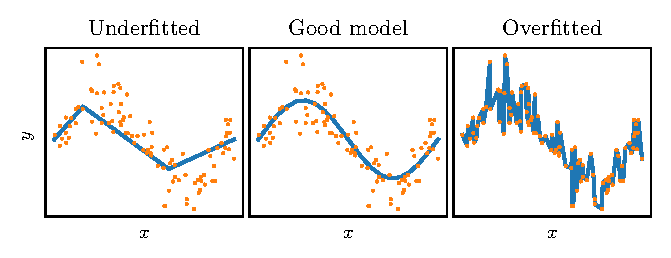
\includegraphics{under_over_train}
    \pause

    \begin{itemize}
        \item Underfitting occurs when you don't train enough for the model to capture the underlying behavior
        \item Overfitting occurs when the training is so good that the neural network memorizes the data, including its underlying noise
        \begin{itemize}
            \item Recall: with enough parameters, neural networks learn anything
        \end{itemize}
    \end{itemize}
\end{frame}

% Including train/validation/test, or put in separate section.
% Under/overfit

%%% Local Variables:
%%% mode: latex
%%% TeX-master: "../nn"
%%% End:

\section{Regularization}

\subsection{}

\begin{frame}
    \frametitle{Underfitting and overfitting}

    \begin{alertblock}{Danger!}
        Neural networks are hard to fit, and real-life data are noisy.
        \emph{Underfitting} and \emph{overfitting} are your two biggest obstacles.
    \end{alertblock}
    \vspace{1ex}

    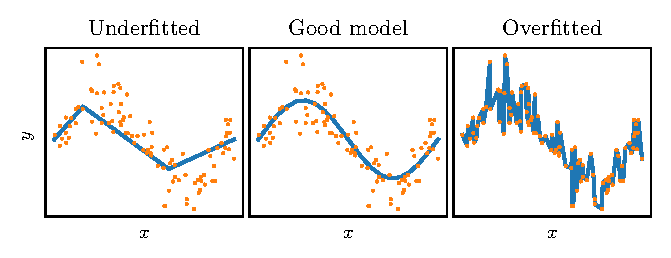
\includegraphics{under_over_train}
    \pause

    \begin{itemize}
        \item Underfitting: didn't train enough for the model to capture the underlying behavior
        \item Overfitting: training so good that neural network memorizes the data, including underlying noise
        \begin{itemize}
            \item Recall: with enough parameters, neural networks learn anything
        \end{itemize}
    \end{itemize}
\end{frame}

\begin{frame}
    \frametitle{Train, validate, test}

    Usual trick: split data into disjoint \textcolor{blue}{training} and \textcolor{Green4}{testing} sets
    \begin{itemize}
        \item Anywhere from 95/5 to 75/25 split is common
        \item Train \emph{only} on the \textcolor{blue}{training set}
        \item Periodically check loss of NN on \textcolor{Green4}{test set}
        \begin{itemize}
            \item Optimizer never sees test set: test set is honest check on NN fidelity
        \end{itemize}
    \end{itemize}
    \pause

    More advanced: split into disjoint \textcolor{blue}{training}, \textcolor{orange}{validation}, and \textcolor{Green4}{testing} set
    \begin{itemize}
        \item Aside on terminology
        \begin{itemize}
            \item Weights \& biases are \alert{parameters}---iteratively improved
            \item Design choices (\# layers, \# neurons, optimizer, \# epochs, etc.) are \alert{hyperparameters}---selected by ML designer
        \end{itemize}
        \item Select different sets of hyperparameters; for each:
        \begin{itemize}
            \item Train only on \textcolor{blue}{training set}, as before
            \item Compute validation loss on \textcolor{orange}{validation set}
        \end{itemize}
        \item Pick hyperparameters with lowest validation loss
        \item Then re-evaluate loss on \textcolor{Green4}{test data}
        \begin{itemize}
            \item Helps remove effects of variance on validation loss
        \end{itemize}
    \end{itemize}
\end{frame}

\begin{frame}
    \frametitle{Training loss vs.\ test loss}
    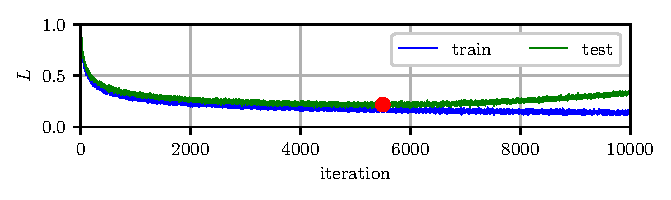
\includegraphics{loss}

    General pattern
    \begin{itemize}
        \item Modulo minor stochastic fluctuations, training loss should monotonically decrease: NN gets better at learning data
        \item Test loss usually at least slightly larger than training loss
        \begin{itemize}
            \item Because optimizer minimizes training loss but never sees test data
        \end{itemize}
        \item At some point, test loss increases: NN overfits to training data
        \item \alert{Early stopping}: use NN with minimum test loss
    \end{itemize}
\end{frame}

\begin{frame}
    \frametitle{Some regularization techniques (1/2)}

    \begin{block}{}
        Regularization: modifications that reduce generalization error
    \end{block}

    \begin{itemize}
        \item<+-> Early stopping
        \item<+-> Don't make NNs too big
        \begin{itemize}
            \item Rule of thumb: $\text{\# parameters} \le \text{\# data}$
        \end{itemize}
        \item<+-> $L^2$ regularization: use loss $\hat{L}(\y, \f(\x; \THETA)) = L(\y, \f(\x; \THETA)) + \alpha \|\THETA\|_2^2$
        \begin{itemize}
            \item Reduces weights, especially in directions that affect $L$ little
        \end{itemize}
        \item<+-> $L^1$ regularization: use loss $\hat{L}(\y, \f(\x; \THETA)) = L(\y, \f(\x; \THETA)) + \alpha \|\THETA\|_1$
        \begin{itemize}
            \item Promotes sparsity in $\THETA$
        \end{itemize}
        \item<+-> Add noise to NN input during training \citep{SietsmaNN91}
        \begin{itemize}
            \item Very non-intuitive to engineers
            \item Prevents overfitting: ``fuzzes'' out bad data
        \end{itemize}
        \item<+-> Bagging (bootstrap aggregating) \citep{BreimanML94}
        \begin{itemize}
            \item For data of size $n$, draw $d$ samples with replacement $m$ times
            \item Train one NN on each of the $m$ sets \& average results
        \end{itemize}
    \end{itemize}
\end{frame}

\begin{frame}
    \frametitle{Some regularization techniques (2/2)}
    \begin{itemize}
        \item<+-> \alert{Dropout} \citep{SrivastavaJMLR14}
        \begin{itemize}[<.->]
            \item During \textcolor{Green4}{training}, randomly remove some portion of connections
            \item Often 20\% of inputs and 50\% of hidden connections
            \item<+-> Put all connections back \& scale accordingly during \textcolor{blue}{inference}
            \item<+-> Motivation: kind of like bagging, but much cheaper
            \item With $n \gg 1$ iterations, essentially average of $n$ models
            \item One of the best regularization techniques; use it!
        \end{itemize}
    \end{itemize}

    \begin{tikzpicture}[node distance=3mm]
    \dropoutnetwork{green}

    \foreach \i/\j in {
        0/1, 0/3, 0/4, 1/0, 1/1, 1/2, 1/4, 2/0, 2/1, 2/2, 2/3, 2/4%
    } {
        \draw (input \i) -- (dense 0\j);
    }

    \foreach \i/\j in {
        0/0, 0/1, 0/2, 1/0, 1/1, 1/2, 1/3, 2/2, 3/0, 3/2, 4/0, 4/1, 4/2%
    } {
        \draw (dense 0\i) -- (dense 1\j);
    }

    \foreach \i/\j in {
        0/0, 1/0, 1/1, 2/1, 3/1%
    } {
        \draw (dense 1\i) -- (output \j);
    }
\end{tikzpicture}
%%% Local Variables:
%%% mode: latex
%%% TeX-master: "../nn"
%%% End:

    \hfill
    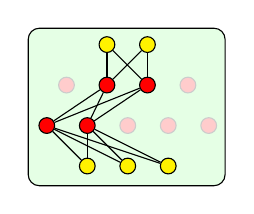
\begin{tikzpicture}[node distance=3mm]
    % Box.
    \draw [fill=green!10, rounded corners] (-0.75, -0.25) rectangle (1.75, 1.75);

    % Nodes.
    \node (input 0) [io mini] {};
    \node (input 1) [io mini, right=of input 0] {};
    \node (input 2) [io mini, right=of input 1] {};

    \node (dense 01) [neuron mini, above=of input 0] {};
    \node (dense 00) [neuron mini, left=of dense 01] {};
    \node (dense 02) [neuron mini off, right=of dense 01] {};
    \node (dense 03) [neuron mini off, right=of dense 02] {};
    \node (dense 04) [neuron mini off, right=of dense 03] {};

    \node (dense 10) [neuron mini off, above=of dense 00, xshift=2.5mm] {};
    \node (dense 11) [neuron mini, right=of dense 10] {};
    \node (dense 12) [neuron mini, right=of dense 11] {};
    \node (dense 13) [neuron mini off, right=of dense 12] {};

    \foreach \i in {0, 1} {
        \pgfmathtruncatemacro{\j}{\i + 1}
        \node (output \i) [io mini, above=of dense 1\j] {};
    }

    % Connections.
    \foreach \i in {0, 1} {
        \foreach \j in {0, ..., 2} {
            \draw (input \j) -- (dense 0\i);
        }

        \foreach \j in {1, 2} {
            \draw (dense 0\i) -- (dense 1\j);
        }
    }

    \foreach \i in {1, 2} {
        \foreach \j in {0, 1} {
            \draw (dense 1\i) -- (output \j);
        }
    }
\end{tikzpicture}
%%% Local Variables:
%%% mode: latex
%%% TeX-master: "../nn"
%%% End:

    \hfill
    \input{figures/dropout3}
    \hfill
    \uncover<2->{\begin{tikzpicture}[node distance=3mm]
    \dropoutnetwork{blue}

    \foreach \i in {0, ..., 4} {
        \foreach \j in {0, ..., 2} {
            \draw (input \j) -- (dense 0\i);
        }

        \foreach \j in {0, ..., 3} {
            \draw (dense 0\i) -- (dense 1\j);
        }
    }

    \foreach \i in {0, 1} {
        \foreach \j in {0, ..., 3} {
            \draw (dense 1\j) -- (output \i);
        }
    }
\end{tikzpicture}
%%% Local Variables:
%%% mode: latex
%%% TeX-master: "../nn"
%%% End:
}

    \begin{itemize}
        \item \alert{Batch normalization} \citep{IoffeICML15}
        \begin{itemize}
            \item Automatically shifts \& scales values to have mean 0 \& variance 1 for each mini-batch
            \item Results in better behavior and easier learning: inputs to activations won't fly to $\pm \infty$
        \end{itemize}
    \end{itemize}
\end{frame}

%%% Local Variables:
%%% mode: latex
%%% TeX-master: "../nn"
%%% End:

\section[CNNs]{Convolutional neural networks}

\subsection{}

\begin{frame}
    \frametitle{Motivation}

    \begin{block}{Disclaimer}
        I know almost nothing about CNNs, but not discussing them would be sacrilegious.
        I'll do my best.
    \end{block}

    \begin{itemize}
        \item Much of deep learning revolves around image classification
        \item A huge proportion of early major breakthroughs in deep learning involved CNNs for image classification
    \end{itemize}

    \begin{block}{Spatial invariance}
        CNNs leverage the fact that images are \alert{spatially invariant}
        \begin{itemize}
            \item A dog is a dog whether its head is in the left or right side of an image
            \item Dense networks treat every input as independent
        \end{itemize}
    \end{block}
\end{frame}

\begin{frame}
    \frametitle{Rich history that authors expect you to know}
    \begin{columns}
        \begin{column}{0.55\textwidth}
            \begin{itemize}
                \item<+-> Late 1990s: MNIST database of handwritten digits
                \begin{itemize}
                    \item 60,000 training samples, 10,000 test samples
                    \item $28 \times 28$ pixels, black and white
                    \item CNN test error: 0.7\% \citep[``LeNet-5'',][]{LeCunIEEE98} to 0.21\% \citep{WanICML13}
                \end{itemize}
                \item<+-> Early 2010s: CIFAR-10/100 database, 10/100 image labels
                \begin{itemize}
                    \item 50,000 training samples, 10,000 test samples
                    \item $32 \times 32$ color images
                    \item CIFAR-10 test error: 35\% \citep{RanzatoAISTATS10} to 2.1\% \citep{Real18}
                \end{itemize}
                \item Early 2010s: ImageNet---$\O(10^7)$ images, $\O(10^4)$ labels
            \end{itemize}
        \end{column}
        \begin{column}{0.45\textwidth}
            \includegraphics[width=\textwidth]{mnist} \\[5mm]
            \uncover<.->{\includegraphics[width=\textwidth]{imagenet}}
        \end{column}
    \end{columns}
\end{frame}

\begin{frame}
    \frametitle{CNN architectures that authors expect you to know}

    Famous architectures + \% test samples with labels not in top 5:
    \begin{itemize}
        \item<+-> LeNet \citep{LeCunIEEE98}: 18.9\% top-5 error
        \begin{itemize}
            \item 2 convolutional layers (size 5, 5) $\to$ 3 dense layers (size 120, 84, 10)
        \end{itemize}
        \item<+-> AlexNet \citep{KrizhevskyNIPS12}: 17.0\%
        \begin{itemize}
            \item 5 convolutional layers (size 11, 5, 3, 3, 3) $\to$ 3 dense layers (size 4096, 4096, 1000)
        \end{itemize}
        \item<+-> ZF Net \citep{ZeilerECCV14}: 11.2\%
        \begin{itemize}
            \item Minor improvement to AlexNet
        \end{itemize}
        \item<+-> VGGNet \citep{Simonyan14}: 7.7\%
        \begin{itemize}
            \item Replace AlexNet's $11 \times 11$ and $5 \times 5$ filters with deep $3 \times 3$ filters
        \end{itemize}
        \item<+-> GoogLeNet/Inception \citep{SzegedyIEEECVPR15}: 6.67\%
        \begin{itemize}
            \item Reduces work by using \emph{Inception modules} that combine size 1, 3, and 5 convolutions
        \end{itemize}
        \item<+-> ResNet \citep{He15b}: 3.57\%
        \begin{itemize}
            \item Instead of feeding convolutional output to next layer, feed convolutional input + output
        \end{itemize}
    \end{itemize}
\end{frame}

%%% Local Variables:
%%% mode: latex
%%% TeX-master: "../nn"
%%% End:

\section[Advice]{General advice}

\subsection{}

\begin{frame}
    \frametitle{Hardware}
    \includegraphics[width=0.48\textwidth]{volta}
    \hfill
    \includegraphics[width=0.48\textwidth]{tpu}

    \begin{itemize}[<+->]
        \item \alert{Use GPUs.}
        The bulk of forward and backprop is matrix--vector multiplies; common for GPUs to be $\O(10 \text{--} 100)\times$ faster than CPUs
        \item \alert{Use GPUs built for NNs.}
        NVIDIA Volta and Google tensor processing unit (TPU) are built from ground-up to be lightning fast for NNs (e.g., 16-bit multiply-add for 32-bit result)
        \item \alert{Use mini-batch sizes and widths that are integer powers of 2.}
        Not a hard rule, but GPUs tend to more efficient this way
        \item \alert{Use 32-bit floats.}
        Neural networks are not turbulence simulations; no tangible benefit to 64-bit doubles
    \end{itemize}
\end{frame}

\begin{frame}
    \frametitle{Software}
    \begin{itemize}
        \item $\exists$ many NN platforms; unclear which will win out in the end.
        \item Most popular now: Keras, TensorFlow, PyTorch
        \begin{itemize}
            \item TensorFlow seems to be winning, but list changes rapidly
        \end{itemize}
        \pause
        \item How do they compare in my opinion?
    \end{itemize}

    \begin{center}
        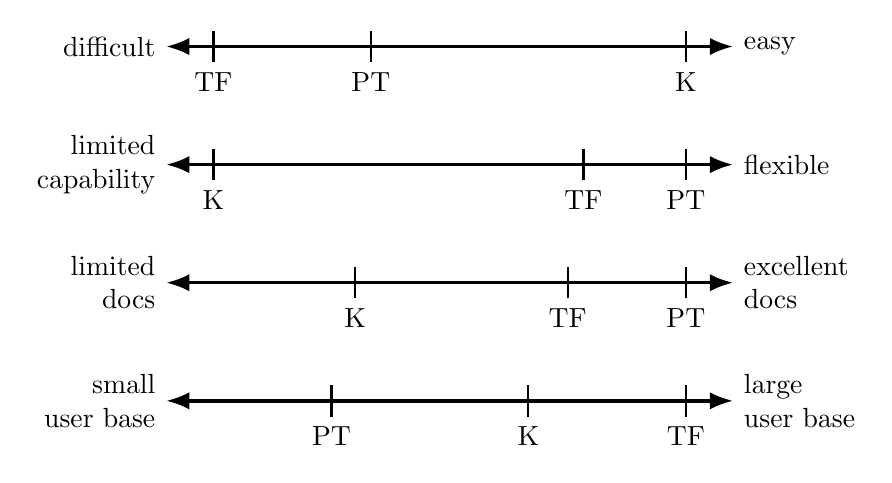
\begin{tikzpicture}
    \def\pos{0}
    \scale{difficult}{easy}
    \entry{TF}{-3}
    \entry{PT}{-1}
    \entry{K}{3}

    \def\pos{-1.5}
    \scale{limited \\ capability}{flexible}
    \entry{K}{-3}
    \entry{TF}{1.7}
    \entry{PT}{3}

    \def\pos{-3}
    \scale{limited \\ docs}{excellent \\ docs}
    \entry{K}{-1.2}
    \entry{TF}{1.5}
    \entry{PT}{3}

    \def\pos{-4.5}
    \scale{small \\ user base}{large \\ user base}
    \entry{PT}{-1.5}
    \entry{K}{1}
    \entry{TF}{3}
\end{tikzpicture}
%%% Local Variables:
%%% mode: latex
%%% TeX-master: "../nn"
%%% End:

    \end{center}
\end{frame}

\begin{frame}
    \frametitle{Neural network architecture}
    \begin{itemize}[<+->]
        \item \alert{Use CNNs for spatial data \& RNNs for temporal data.}
        \item \alert{Start with architectures that are too small.}
        NNs take a long time to train; make problems show up immediately.
        \item \alert{Scale up architectures until they overfit.}
        Check the relation between NN size and validation loss.
        Back off on size if validation loss increases.
        \item \alert{Use pretraining.}
        If applicable, borrow NN architecture from pre-existing model (e.g., ResNet), and initialize parameters to trained values from different task.
        \item \alert{Use dropout.}
        They are one of the best regularizers.
        \item \alert{Aim for $\text{\# parameters} \le \text{\# data}$.}
        Helps prevent overfitting.
        \item \alert{Set layer $i$ to be \sfrac{1}{2}--\sfrac{3}{4} the width of layer $i - 1$.}
        Layers closer to the input have greater expressive power.
        \item \alert{Beware of excessive depth.}
        They make NNs much harder to train and can cause overfitting.
    \end{itemize}
\end{frame}

\begin{frame}
    \frametitle{End-to-end machine learning}

    \begin{block}{}
        \alert{End-to-end}: give the model input \& output data, but don't tell it how to get from inputs to outputs.
        Let the model figure it out.
    \end{block}

    \begin{center}
        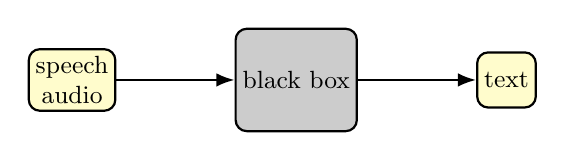
\begin{tikzpicture}[node distance=1.5cm]
    \node (audio) [draw, block, fill=yellow!20, align=center] {speech \\ audio};
    \node (box) [draw, block, fill=black!20, minimum height=1.3cm, minimum width=1.3cm, align=center, right=of audio] {black box};
    \node (text) [draw, block, fill=yellow!20, right=of box] {text};

    \draw [path] (audio) -- (box);
    \draw [path] (box) -- (text);
\end{tikzpicture}

%%% Local Variables:
%%% mode: latex
%%% TeX-master: "../nn"
%%% End:

    \end{center}
    \pause

    \begin{block}{}
        Alternative: define intermediate variables; train models from inputs to intermediate variables to outputs
    \end{block}

    \begin{center}
        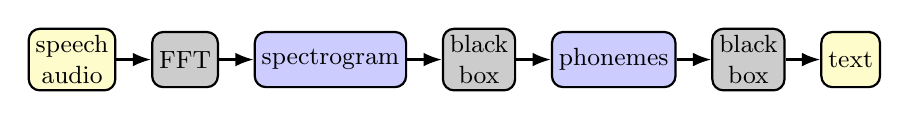
\begin{tikzpicture}[node distance=4.4mm]
    \node (audio) [draw, block, fill=yellow!20, align=center] {speech \\ audio};
    \node (box 0) [draw, block, fill=black!20, right=of audio] {FFT};
    \node (spectrum) [draw, block, fill=blue!20, right=of box 0] {spectrogram};
    \node (box 1) [draw, block, fill=black!20, align=center, right=of spectrum] {black \\ box};
    \node (phonemes) [draw, block, fill=blue!20, right=of box 1] {phonemes};
    \node (box 2) [draw, block, fill=black!20, align=center, right=of phonemes] {black \\ box};
    \node (text) [draw, block, fill=yellow!20, right=of box 2] {text};

    \draw [path] (audio) -- (box 0);
    \draw [path] (box 0) -- (spectrum);
    \draw [path] (spectrum) -- (box 1);
    \draw [path] (box 1) -- (phonemes);
    \draw [path] (phonemes) -- (box 2);
    \draw [path] (box 2) -- (text);
\end{tikzpicture}

%%% Local Variables:
%%% mode: latex
%%% TeX-master: "../nn"
%%% End:

    \end{center}
    \pause

    \begin{itemize}
        \item End-to-end can learn very complex input--output relations\ldots
        \item But requires enormous data and very powerful models/optimizers
        \item Often best not to start with end-to-end
    \end{itemize}
\end{frame}

\begin{frame}
    \frametitle{Data}

    \begin{itemize}
        \item<+-> \alert{Normalize the data, or use batch normalization.}
        NNs learn better if inputs look standard normal and uncorrelated.
        \item<+-> \alert{Don't extrapolate.}
        Models are meaningless outside their domain of training.
        \begin{itemize}
            \item E.g., sigmoid/ReLU activations have 0th/1st order extrapolation
        \end{itemize}
    \end{itemize}

    \begin{columns}
        \begin{column}{0.4\textwidth}
            \centering
            \footnotesize

            \visible<+->{
                \includegraphics[width=1.5in]{ripple} \\
                ground truth, $[-12, 12] \times [-12, 12]$
            }
            \visible<+->{
                \includegraphics[width=1.5in]{extended_ripple} \\
                ground truth, $[-18, 18] \times [-18, 18]$
            }
        \end{column}

        \begin{column}{0.6\textwidth}
            \centering
            \footnotesize

            \setcounter{beamerpauses}{3}
            \visible<+->{
                \includegraphics[width=1.5in]{ripple_2layer} \\
                17--8 neurons, $[-12, 12] \times [-12, 12]$
            }
            \visible<+->{
                \includegraphics[width=1.5in]{extrapolated_ripple} \\
                above model extrapolated to $[-18, 18] \times [-18, 18]$
            }
        \end{column}
    \end{columns}
\end{frame}

\begin{frame}
    \frametitle{Engaging with the scientific community}

    \begin{itemize}
        \item<+-> \alert{Stay on top of recent conferences and arXiv papers.}
        Papers seem to become obsolete after 2 years.
        \item<+-> \alert{Be aware of \emph{interpretability} criticisms, but do not fear them.}
        \begin{itemize}[<+->]
            \item Main reason physicists reject machine learning: \\[1ex]

            \emph{``So you made a model with 1,000,000,000 parameters, and you fit the data, but you haven't a clue what any of those parameters actually means, or why your model does what it does.''} \\[1ex]

            \ldots or something like that
            \item ML community divided on whether interpretability is important
            \item But don't ignore the results: \emph{ML works}, whether you understand its inner workings or not
            \item<.-> (I drive a car everyday, and I understand its behavior, but I have no idea how it works)
        \end{itemize}
    \end{itemize}
\end{frame}

%%% Local Variables:
%%% mode: latex
%%% TeX-master: "../nn"
%%% End:

\footnotesize

\begin{frame}[allowframebreaks]{References}
    \bibliography{nn}
\end{frame}

%%% Local Variables:
%%% mode: latex
%%% TeX-master: "../nn"
%%% End:


\end{document}

%%% Local Variables:
%%% mode: latex
%%% TeX-master: t
%%% End:
